\documentclass[]{lapesd-thesis}

% Outros \usepackage{}

%%%%%%%%%%%%%%%%%%%%%%%%%%%%%%%%%%%%%%%%%%%%%%%%%%%%%%%%%%%%%%%%%%%%
%%% Configurações da classe (dados do trabalho)                  %%%
%%%%%%%%%%%%%%%%%%%%%%%%%%%%%%%%%%%%%%%%%%%%%%%%%%%%%%%%%%%%%%%%%%%%

% Informações para capa e folha de rosto/certificacao
\titulo{Template \LaTeX{} para testes e dissertações do LAPESD/UFSC}
\autor{Omar Ravenhurst}
\data{1 de agosto de 2019} % ou \today
\tese % ou \dissertacao
\titulode{Doutor em Ciência da Computação}
\orientador{Prof. Ben Trovato, Dr.}
\coorientador{Prof. Lars Thørväld, Dr.}

%%% Atenção! No caso de TCC, além de usar \tcc, outros comandos devem ser 
%%% fornecidos:
% \tcc
% \departamento{Departamento de Informática e Estatística}
% \curso{Ciência da Computação}
% \titulode{Bacharel em Ciência da Computação}
% %% Para TCCs, orientadores e coorientadores podem ser externos, logo a
% %% BU exige que sua afiliação seja explicitada. Por padrão, assume-se
% %% UFSC. Você pode alterar a afiliação com os comandos abaixo:
% \afiliacaoorientador{Universidade Federal de Santa Catarina}
% \afiliacaocoorientador{Universidade Federal da Terra de Ninguém}

% Membros da banca e coordenador
% As regras da BU agora exigem que Dr. apareça depois do nome
% Dica: para gerar Profᵃ. use Prof\textsuperscript{a}.
% Dica 2: para feminino use \orientadora e \coorientadora
\membrobanca{Prof. Valerie Béranger, Dr.}{Universidade Federal de Santa Catarina}
\membrobanca{Prof. Mordecai Malignatus, Dr.}{Universidade Federal de Santa Catarina}
\membrobanca{Prof. Huifen Chan, Dr.}{Universidade Federal de Santa Catarina}
\coordenador{Prof. Charles Palmer, Dr.}


% Ativa indíce remissivo. Precisa estar aqui, não funciona no .cls nem no
% \BeforeBeginDocument{}
\makeindex
% Carrega definições dos acrônimos e do glossário. Isso precisa ser feito antes
% do \begin{document}

%%%%%%%%%%%%%%%%%%%%%%%%%%%%%%%%%%%%%%%%%%%%%%%%%%%%%%%%%%%%%%%%%%%%
%%% Lista de acronimos                                           %%%
%%%%%%%%%%%%%%%%%%%%%%%%%%%%%%%%%%%%%%%%%%%%%%%%%%%%%%%%%%%%%%%%%%%%
%%% Importante:                                      
%%% - A lista PRECISA SER MANTIDA ORDENADA
%%%%%%%%%%%%%%%%%%%%%%%%%%%%%%%%%%%%%%%%%%%%%%%%%%%%%%%%%%%%%%%%%%%%

\tnewacronym{API}{Application Programming Interface}
            % \API e \APIs nunca espandem, mas ele aparece na lista de siglas
\xnewacronym{DHT}{Distributed Hash Table}
            % Se \DHTs for o primeiro uso, Tabe ganha um s no final
\xnewacronym[][longplural={Square Matrices}]{SQ}{Square Matrix}
               % trata o plural usado em \SQs
               % note que como queremos passar o 2o arg opcional, devemos 
               % passar o primeiro (podemos deixar em branco)
\xnewacronym[WTC]{W3C}{World Wide Web Consortium}
            % gera comando \WTC que expande para "World ... (W3C)"

%%% Local Variables:
%%% mode: latex
%%% TeX-master: "main"
%%% End:


%%%%%%%%%%%%%%%%%%%%%%%%%%%%%%%%%%%%%%%%%%%%%%%%%%%%%%%%%%%%%%%%%%%%
%%% Glossario                                                    %%%
%%%%%%%%%%%%%%%%%%%%%%%%%%%%%%%%%%%%%%%%%%%%%%%%%%%%%%%%%%%%%%%%%%%%
%%% Importante:                                      
%%% - A lista PRECISA SER MANTIDA ORDENADA
%%%%%%%%%%%%%%%%%%%%%%%%%%%%%%%%%%%%%%%%%%%%%%%%%%%%%%%%%%%%%%%%%%%%

\xnewglossaryentry{polling}{%
  name={polling},%
  description={A type of event delivery technique consisting of the consumer repeatedly asking the provider for the most recent events}%
}
\xnewglossaryentry{proxy}{%
  name={proxy},%
  plural={proxies},%
  description={A proxy \cite[p.~3]{shapiro1986} encapsulates remote servers and provides a single view to their services. The proxy can then intercept communication and provide additional functionality, such as message translation and performance enhancement. The client must take the initiative of selecting and using a proxy \cite[p.~46,97]{fielding2000}.}%
}

%%% Local Variables:
%%% mode: latex
%%% TeX-master: "main"
%%% End:


\begin{document}

%%%%%%%%%%%%%%%%%%%%%%%%%%%%%%%%%%%%%%%%%%%%%%%%%%%%%%%%%%%%%%%%%%%%
%%% Conteúdo                                                     %%%
%%%%%%%%%%%%%%%%%%%%%%%%%%%%%%%%%%%%%%%%%%%%%%%%%%%%%%%%%%%%%%%%%%%%

\pretextual%
% Assume-se que \pretextual já foi feito


\imprimircapa%
\imprimirfolhaderosto*
% Atenção! esse \protect é importante
\protect\incluirfichacatalografica{ficha.pdf}
\imprimirfolhadecertificacao


\begin{dedicatoria}
  Este trabalho é dedicado à wikipedia e ao stackoverflow. Essa frase está aqui apenas para testar o alinhamento e as margens
\end{dedicatoria}


\begin{agradecimentos}
  O presente trabalho foi realizado com apoio da Coordenação de Aperfeiçoamento de Pessoal de Nível Superior -- Brasil (CAPES) -- Código de Financiamento 001.
\end{agradecimentos}


\begin{epigrafe}
  For a number of years I have been familiar with the observation that the quality of programmers is a decreasing function of the density of go to statements in the programs they produce \\
  \cite{dijkstra1968}
\end{epigrafe}


\begin{resumo}[Resumo]
  Aqui deve ser inserido um resumo de 150 a 500 palavras (limitação de tamanho dada pela BU). A linguagem deve ser português e a hifenização já foi alterada. O resumo em português deve preceder o resumo em inglês, mesmo que o trabalho seja escrito em inglês. A BU também diz que deve ser usada a voz ativa e o discurso deve ser na 3ª pessoa. A estrutura do resumo pode ser similar a estrutura usada em artigos: Contexto -- Problema -- Estado da arte -- Solução proposta  -- Resultados.

  % Atenção! a BU exige separação através de ponto (.). Ela recomanda de 3 a 5 keywords
  \vspace{\baselineskip} 
  \textbf{Palavras-chave:} Palavra-chave. Ponto como separador. Bla.
\end{resumo}


\begin{resumo}[Resumo Estendido]
%%%%%%%%%%%%%%%%%%%%%%%%%%%%%%%%%%%%%%%%%%%%%%%%%%%%%%%%%%%%%%%%%%%%%%
% Atenção: normas e templates contraditórios!!!                    %%%
%%%%%%%%%%%%%%%%%%%%%%%%%%%%%%%%%%%%%%%%%%%%%%%%%%%%%%%%%%%%%%%%%%%%%%
% - Modelo da BU: https://repositorio.ufsc.br/handle/123456789/197458
% - A BU exige no **mínimo** 2 páginas e no **máximo** 5
% - Regimento do PPGCC, Art 40 Entende-se  por  resumo  estendido  um  documento  que  contenha  as  informações  mais  relevantes  de  cada  capítulo  da  tese  ou  da  dissertação.
% O mais seguro é ignorar o regimento e seguir a BU.
    % Atenção! A BU diz que o resumo **deve** conter as seções abaixo!
  \section*{Introdução} % Deve ser  subsection*, devido a formatação usada no modelo
  A hifenização é alterada para \texttt{brazil}, mesmo para documentos em inglês. Descrever brevemente esses itens exigidos pela BU. Como a RN 95/CUn/2017 é mais recente e impõe outras regras a revelia de regimentos e regulamentos, é mais sábio obedecê-la. Lembre que esse resumo estendido deve term entre 2 e 5 páginas.
  
  \lipsum[1]
  \section*{Objetivos} 
  \lipsum[21]
  \section*{Metodologia} 
  \lipsum[3]
  \section*{Resultados e Discussão} 
  \lipsum[4]
  \section*{Considerações Finais} 
  \lipsum[5]

  \vspace{\baselineskip}  % Atenção! manter igual ao resumo
  \textbf{Palavras-chave:} Palavra-chave. Outra Palavra-chave composta. Bla.
\end{resumo}


\begin{abstract}
  Enlish version of the plain ``resumo'' above. Hyphenization is automatically changed to english

  \vspace{\baselineskip} 
  \textbf{Keywords:} Keyword. Another Compound Keyword. Bla.
\end{abstract}

\listoffigures*  % O * evita que apareça no sumário
\listoftables*
\listoflistings*  
\listofalgorithms*

\listadesiglas*

\begin{listadesimbolos}
  $\gets$   & Atribuição \\
  $\exists$   & Quantificação existencial \\
  $\rightarrow$   & Implicação \\
  $\wedge$   & E lógico \\
  $\vee$   & Ou lógico \\
  $\neg$   & Negação lógica \\
  $\mapsto$   & Mapeia para \\
  $\sqsubseteq$   & Subclasse (em ontologias) \\
  $\subseteq$   & Subconjunto: $\forall x\;.\; x \in A \rightarrow x \in B$ \\
  $\langle\ldots\rangle$ & Tupla \\
  $\forall$   & Quantificação universal \\
  mmmmm & Nenhum sentido, apenas estou aqui para demonstrar a largura máxima dessas colunas. Ao abrir o ambiente \texttt{listadesimbolos}, pode-se fornecer um argumento opcional indicando a largura da coluna da esquerda (o default é de 5em): \texttt{\textbackslash{}begin\{listadesimbolos\}[2cm] .... \textbackslash{}end\{listadesimbolos\}} \\
\end{listadesimbolos}

\tableofcontents*%

%%% Local Variables:
%%% mode: latex
%%% TeX-master: "main"
%%% End:

\textual%
% Assume-se que \textual já foi feito

\chapter{Exemplo}
\label{ch:exemplo}

\index{bobagem} Primeiro parágrafo da seção com uma frase sem sentido que só serve para ocasionar uma quebra e de demonstrar a configuração de indentação da primeira linha. Essa frase está aqui pois parágrafos de uma linha são feios.

Resultado do uso de siglas:
\begin{itemize}
\item Sigla que nunca expande: \API;
\item Sigla normal, expande no primeiro uso: \DHT, mas não no segundo: \DHT;
\item Siglas com plurais automaticos: \APIs e \DHTs;
\item Plural não-trivial: \SQs;
\item Forçando uma expansão (e no plural) \Glsfirstplural{DHT};
\item Usando uma sigla cujo comando é diferente da sigla: \WTC.
\end{itemize}

Resultado do glossário:
\begin{itemize}
\item Dois termos, \polling e \proxy;
\item Plural: \proxys.
\end{itemize}

Resultado de \mla|index|: primeiro um link normal \indexterm{tomate}, depois um capitalizado \indexTerm{tomate}.

Exemplo de autoref com \mla|amsthm|: \autoref{def:definition}, \autoref{def:defn}, \autoref{lemma:1}, \autoref{theorem:1}, \autoref{proof:1}.

\begin{definition}
  \label{def:definition}
  Exemplo de definição.
\end{definition}

\begin{defn}
  \label{def:defn}
  Exemplo de definição com ambiente defn.
\end{defn}

\begin{lemma}
  \label{lemma:1}
  Exemplo de Lema.
\end{lemma}

\begin{theorem}
  \label{theorem:1}
  Exemplo de teorema.
  \begin{proof}
    Exemplo de prova dentro do teorema \qed
  \end{proof}
\end{theorem}

\begin{theoremproof}
  \label{proof:1}
  Exemplo de prova \qed
\end{theoremproof}

(Sub)enumerações e citações (verificar se OK com o idioma):
\begin{enumerate}
\item \cite{turing1937}:
  \begin{enumerate}
  \item \citeonline{turing1937}:
    \begin{enumerate}
    \item \citeonline{dijkstra1968};
    \end{enumerate}
  \end{enumerate}
\item \cite{turing1937,dijkstra1968};
\item \citeonline{turing1937,dijkstra1968}.
\end{enumerate}


\begin{listing}[tb]
\caption{Meta informações do presente documento.}
\label{lst:meta}
\begin{minted}[highlightlines={1,4-5}]{latex}
\titulo{Template \LaTeX{} para testes e dissertações do LAPESD/UFSC}
\autor{Omar Ravenhurst}
\data{1 de agosto de 2019} % ou \today
\tese % ou \dissertacao
\titulode{Doutor em Ciência da Computação}
\orientador{Prof. Ben Trovato, Dr.}
\coorientador{Prof. Lars Thørväld, Dr.}

\membrobanca{Prof. Valerie Béranger, Dr.}{Universidade Federal de Santa Catarina}
\membrobanca{Prof. Mordecai Malignatus, Dr.}{Universidade Federal de Santa Catarina}
\membrobanca{Prof. Huifen Chan, Dr.}{Universidade Federal de Santa Catarina}
\coordenador{Prof. Charles Palmer, Dr.}
\end{minted}
\fonte{o autor.}
\end{listing}


Resultado de \mla|\autoref|s:
\begin{itemize}
\item \autoref{lst:meta};
\item \autoref{alg:algoritmo};
\item \autoref{fig:figura} tem subfiguras:
  \begin{itemize}
  \item \autoref{fig:svg}
  \item \autoref{fig:brasao}
  \end{itemize}
\item \autoref{tb:tabela};
\item \autoref{ch:exemplo};
\item \autoref{sec:frutas};
\item \autoref{sec:goiaba};
\item \autoref{sec:jabuticaba};
\item \autoref{sec:tomate}.
\end{itemize}


\begin{algorithm}
  \caption{Exemplo do ambiente \texttt{algorithimic}.}
  \label{alg:algoritmo}
  \begin{algorithmic}[1]
    \Procedure{Closure}{C, A}
      \State{$H \gets \emptyset$}\Comment{Direct cache}
      \For{$i \in [1, n]$}\Comment{Parallel, (dynamic,32) scheduling}
        \State{$H \gets H \cup \Call{DoImportantStuff}{i}$}
      \EndFor
    \EndProcedure
  \end{algorithmic}
  \fonte{o autor.}
\end{algorithm}

\begin{figure}[tb]
  \centering
  \caption{Exemplo de figura com duas subfiguras.}   
  \label{fig:figura}
  
  % Subfiguras são feitas usando as funcionalidades do memoir. Não
  % inclua outros pacotes, pois eles podem fazer o memoir dar ragequit
  % 
  % Há duas maneiras, a maneira limpinha (só no lapesd-thesis.cls) e a
  % maneira do memoir (aviso: \subtop não funciona direito).
  \subcaptionminipage[fig:svg]%
    {.49\linewidth}%
    {O Makefile compila SVGs em PDFs usando o inkscape}%
    {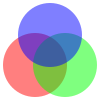
\includegraphics[width=.2\linewidth]{alphachannel.pdf}}%
  \hfill% 
  % o comando acima expande para o equivalente disso:
  \begin{minipage}[t]{.49\linewidth}%
    \centering
    \subcaption{Brasão da UFSC.\label{fig:brasao}}
    \includegraphics[width=.2\linewidth]{\jobname-logo.pdf}
  \end{minipage}

  \fonte{o autor.}
\end{figure}

\begin{table}[tb]
  \centering
  \caption{Exemplo de tabela e símbolos}
  \label{tb:tabela}
  \begin{tabular}{lccp{5cm}}
    \toprule
    Esquerda & Coluna 1    & \rotatebox{90}{90 graus}  & Parágrafo com \mla|p{5cm}|   \\
    \midrule
    $r_1$    & \cmk        &  \xmk                     & \circledi    \\
    $r_2$    &     \multicolumn{2}{c}{merged cell}     & \circledii   \\
    $r_3$    & \circlediii & \circlediv                & \circledv    \\
    $r_4$    & \circledvi  & \circledvii               & \circledviii \\
    $r_5$    & \circledix  &  x                        & y           \\
    \bottomrule 
  \end{tabular}
  \fonte{o autor.}
\end{table}

\section{Frutas}
\label{sec:frutas}
\lipsum[4]

\subsection{Goiaba}
\label{sec:goiaba}
\lipsum[4]

\subsubsection{Jabuticaba}
\label{sec:jabuticaba}
\lipsum[4]

\subsubsubsection{Tomate}
\label{sec:tomate}

\begin{figure}[tb]
  \centering
  \caption{Segunda Figura.}
  \label{fig:segunda-fig}
  \includegraphics[width=.2\linewidth]{\jobname-logo.pdf}
  \fonte{o autor.}
\end{figure}

\xindex{tomate} \lipsum[4]


%%% Local Variables:
%%% mode: latex
%%% TeX-master: "main"
%%% End:

\postextual
% Assume-se que \postextual já foi feito

\imprimirglossario

\apendices

\chapter{Exemplo de Apêndice}
\label{ch:apendice}

% Uso de \cite em apêndice/anexo como se fossem antes do \bibliography{}.  NBR
% 14724 e NBR 6023, assim como os documentos da BU não especificam nada sobre
% citações dentro de apêndices/anexos. No entanto, em email trocado com a BU, a
% orientação foi de usar \cite{} normalmente e deixar que as referências sejam
% listadas na única bibliografia do documento, mesmo que esta esteja antes dos
% apêndices. A argumentação é que apêndices e anexos são numerados e fazem parte
% do documento, logo suas referências devem ser listadas como referências do
% documento. Além disso as normas não prevem segmentar as referências por
% capítulos.
\cite{turing1937} \lipsum[1] 

\imprimirindice


%%% Local Variables:
%%% mode: latex
%%% TeX-master: "main"
%%% End:


\bibliography{main}

\end{document}
